\chapter{Method}
\label{chap:2}

\section{The UNEP Campaign}
The United Nations environment programme (UNEP) measurement campaign aimed to quantify the total type-based (natural and anthropogenic) methane emissions of Hamburg \cite{Forstmaier.2023}. Three measurement types were deployed during this campaign. A total column-based Fourier-Transform Infrared Spectrometer network, deployed from 27.07.2021 to 9.09.2021. A continuous flow isotope ratio mass spectrometer (IRMS) measurement at the Geomatikum from 01.08.2021 to 1.04.2022, a mobile dual Cavity Ring-Down Spectrometer measurements by car and boat from 09.08.2021 to 21.08.2021.\\
The FTIR sensor network is part of the Munich Urban Carbon Column Network (MUCCnet) and was relocated for the measurement campaign to Hamburg. The coordination and deployment were provided by the Technische Universität München (TUM) from Andreas Forstmaier (TUM) and Jia Chen (TUM). The sensors used in the MUCCnet are solar-tracking absorption spectrometers (Bruker, EM27/SUN) that enable column-averaged dry air mole fractions measurements of CO$_2$, CH$_4$, and O$_2$ \cite{Chen.2016}. A Bayesian inverse modelling approach was used to estimate the location and type-based methane emissions. The TNO GHGco inventory (Super et al. [2020]) was used as Prior information for the Bayesian approach. The inventory was further improved for the modelling by the results of the mobile survey. The ERA5 model \cite{Hersbach.2023} was used to model the transport by the atmosphere. The Wind lidar measurements were used to correct this model further. The wind lidar deployed was the Leosphere Windcube 200S Doppler wind LIDAR provided and operated by Norman Wildmann from the Deutsches Zentrum für Luft- und Raumfahrt (DLR) \cite{Wildmann.2020}, \cite{Vasiljevic.2016}.\\
The Isotope Ratio Mass Spectrometer system at the Geomatikum was provided by the Universiteit Utrecht and operated by Carina van der Veen. The Spectrometer used was a ThermoFinnigan MAT Deltaplus XL isotope ratio mass spectrometer, alternating $^2$H and $^{13}$C measurements with a frequency of 20 min. The measured Isotope ratios were analysed using a Keeling plot approach and compared for identification to a stable isotope ratio database of isotope measurements of known source types \cite{Menoud.2021}. \\
The mobile measurement survey deployed two Cavity Ring-Down Spectrometers, the Picarro model G2301 and a Picarro model G4302. Additionally, methane plumes were analysed by sample bags for their source attribution. The bags were examined with the isotope ratio spectrometer in the Geomatikum. Hossein Maazallahi from the Universiteit Utrecht conducted the mobile measurement survey. The survey completed a previous campaign performed with the same instrumentation in 2020 \cite{Maazallahi.2020}, concentrating on the northern parts of Hamburg, primarily residential areas. The measurements conducted between 09.08.2021 and 21.08.2021 focused on the southern regions with mostly industrial and port areas, surveying 1567 km.

\section{Continuous-flow isotope ratio mass spectrometry (CF-IRMS)}
The isotopic ratio signatures of Deuterium ($\delta$D) and Carbon-13 ($\delta ^{13}$C) were measured by using a continuous flow Isotopic Ratio Mass Spectrometer (CF-IRMS).  Isotope measurements are well suited to provide additional information about the production mechanism of methane since different sources emit CH$_4$ with a characteristic and, in many cases, distinct isotopic composition.\\
The system used is described in great detail by \cite{Brass.2010}, nether the less the analysis method is briefly described here to give a general inside. The method used is designed for a multi-month operation with minimal user interaction. Apart from liquid nitrogen refilling, which is used for cooling, the process is fully automated and continuously measures autonomously. Besides a few short 1-3 day maintenance beaks in which the furnace had to be replaced, the setup measured uninterrupted for the extended time period from 01.08.2021 to 1.04.2022. The isotope ratio determination procedure follows seven steps based on extracting and purifying the methane before analysing it with the mass spectrometer. \cite{Brass.2010}.
\begin{enumerate}
  \item In the first step, the air is sampled with a fixed volume of 40 mL.
  \item The methane is then pre-concentrated. This separates the methane from the bulk air. The separation process is performed by cooling the air to -130 °C. At this temperature, CH$_4$ condensates while N$_2$ and O$_2$ stay gaseous and can be separated mechanically. The remaining air is then heated to -85 °C, where the CH$_4$ becomes a gas again, but N$_2$, O$_2$, CO$_2$, H$_2$O and other condensable gases stay solid/liquid and are again mechanically separated by valves.
  \item The CH4 is focused in a small volume by recooling the methane. This also ensures a better separation from the O$_2$, N$_2$, and CO$_2$, which can harm the conditioning of the furnaces or cause interferences in the mass spectrometer. By reheating the CH$_4$, the release peak can be shortened, which ensures a high enough concentration in later processes. 
  \item The CH$_4$ is gas chromatographically separated by a PoraPLOT Q column from the remaining gas components.
  \item CH$_4$ is converted to either CO$_2$ or H$_2$, the two processes are alternated with a 20 min frequency. The CH$_4$ is combusted into CO$_2$ for the ${^{13}C}/{^{12}C}$ ratio analysis. In this process, the CH$_4$ is broken into CO$_2$+ H$_2$O. For the ${^{2}H}/{^{1}H}$ ratio analysis, the CH4 is converted to C+ 2H$_2$ via pyrolysis. This process uses highly purified Helium (He) (purity 5.0) as a transport medium.
  \item The converted CH4 is injected into the mass spectrometer via an open split interface 
  \item The mass spectrometer measures the molecular ion current ratios. The peak areas are evaluated for a methane concentration analysis.
\end{enumerate}
\begin{figure}[htbp]
 \centering
 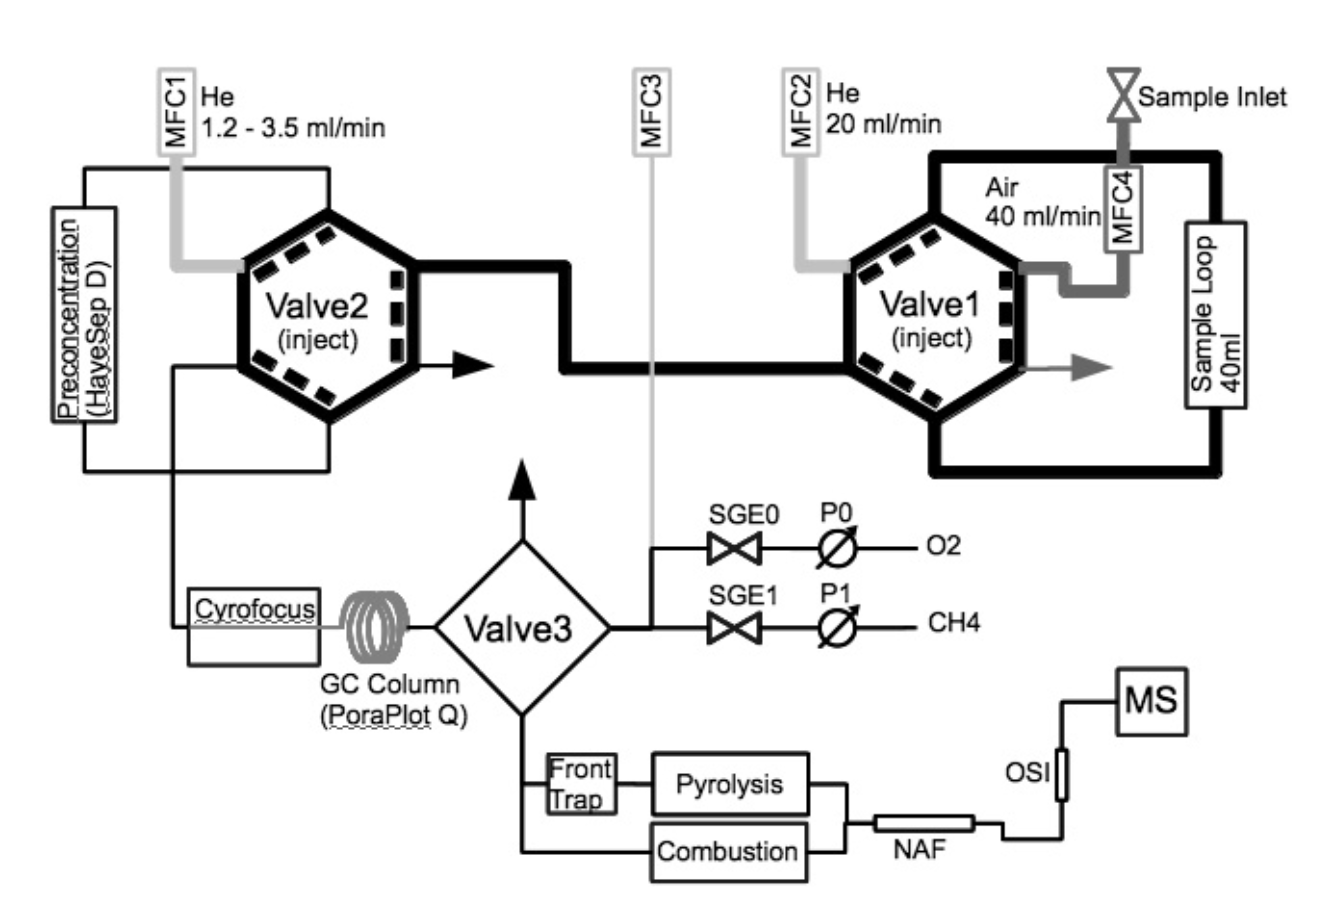
\includegraphics[width=1\textwidth]{figures/Methode/CF-IRMS_schematics.png}
 \caption[CF-IRMS schematics]{Schematics for the Continuous-flow isotope ratio mass spectrometry (CF-IRMS) deployed at the Geomatikum. Methane is isolated from other air components by subsequent preconcentration, cryo-focussing and gas chromatographic separation. The separated methane is then either combusted to CO$_2$ (for ${^{13}C}/{^{12}C}$ ratio analysis) or pyrolyzed to H$_2$ (for ${^{2}H}/{^{1}H}$ ratio analysis) and injected into the isotope ratio mass spectrometer for isotopic analysis. \cite{Brass.2010}}
 \label{CFIRMSSschematics}
\end{figure}
For calibration and stability monitoring, the isotopic ratio mass spectrometer measurement is packaged into six individual measurements (Reference-Sample-Sample-Sample-Sample-Reference). A complete measurement cycle takes About 20 minutes, and the $\delta ^{13}$C and $\delta$D measurements are alternated. The system pressure is also measured with a pressure sensor to determine the methane concentration of the sample air.

\subsection{Mass Spectroscopy}
The commonly used analytical technique of mass spectroscopy offers an excellent tool for measuring ion mass to charge ratio. This allows for accurate measurement of the isotope ratios in a sample, giving great insight into the production mechanisms of the molecules studied. By measuring and analysing the ratios of Hydrogen ($^{1}H$) to its heavier Deuterium ($^{2}H$) isotope and Carbon ($^{12}$C) to its heavier Carbon-13 ($^{13}$C) Isotopes in methane, its origin can be estimated. Further detail on this analysis process will be given later in the section on Keeling plot analysis.\\
A mass spectrometer can measure the charge ratio of an uncharged molecule by ionising the molecule by electron impact. The ionised molecule now has an electric potential and can experience the effects of magnetic and electrostatic fields.\\
The ions are accelerated using an electric potential, resulting in a similar Kinetic energy for all ions independent of their mass-to-charge ratio.\\
A magnetic field ($B$) is then applied to the accelerated ions resulting in a Lorenz force experienced by the ions. Consequently, the trajectory of the ions is bent towards a circle within the magnetic field. While equal charges ($q$) with an equal velocity ($v$) experience the same Lorenz force, they do not necessarily follow the same Circular trajectory and have the same radius ($r$). This is co-dependent on the mass ($m$) of the charge, i.e. the ionised molecule or atom. Hence for isotopes with larger masses, the radius of the trajectory differs from the radius of the lighter parent isotope. The heavier isotopes have a larger radius than their lighter contra part.
\begin{equation}
\frac{m}{q} = \frac{r \times B}{v^2}
\end{equation}
A continuous flow of ions on the magnetic field generates a mass spectrum on a detector (Ion collectors), a histogram of the isotope abundance/intensity versus its mass-to-charge ratio.\\
The mass spectrometer measures the Isotope ratio $\delta$X, which is noted in $\permil$. The isotope ratio describes the ratio of two isotopes ($R = {^{13}C}/{^{12}C} \ or \ R = {^{2}H}/{^{1}H}$) in a sample relative to the same ratio in a reference/standard material. 
\begin{equation}
\delta X = \frac{R_{sample} - R_{standard}}{R_{standard}}
\end{equation}
Due to the high cost and scarcity of well-defined and peer-reviewed reference samples, the measurements are performed against a working standard (WS). This Working standard is calibrated to a small amount of a well-defined reference with the mass spectrometer that will be used in the sample measurements.
The measured Isotope ratio of the sample can, later on, be converted to the international isotope scale (IS)by: 
\begin{equation}
\delta_{\frac{sample}{IS}} = \delta_{\frac{WS}{IS}} \delta_{\frac {sample}{WS}} + \delta_{\frac {WS}{IS}} + \delta_{\frac {sample} {WS}}
\end{equation}
The measurement results can then be published on the international isotope scale. The uncertainty in the reference sample and the instruments have to be accounted for when such an approach is implemented. For $^{13}$C
the international Isotope scale is the Viana Pee Dee Belemnite(VPDB), and for $^{2}H$, the IS is the Vienna Standard Mean Ocean Water (VSMOW).\\
By comparing the area of an isotope peak in the mass spectrum in the sample to a well-calibrated working standard reference of this spectrometer, the concentration can be calculated as follows:
\begin{equation}
c_{sample} = c_{WS} \frac{peak\  area_{sample}}{peak\  area_{WS}}
\end{equation}

\subsection{Keeling plot methode}
%needs rewriting!!!!!!
%%%%%%%references!!!!!!!!!!!!!!!
Charles D. Keeling showed in the fifties that the isotopic abundance of $ ^{13}C$ and $^{18}O$ can be correlated to the plant-based origin of CO$_2$ \cite{CharlesDKeeling.1958}, \cite{CharlesDKeeling.1960}. He devised a method for estimating the production mechanism of CO$_2$ by reference databases. This method was later adopted for methane. The abundance of heavy isotopes of 13C and 2H in a methane molecule enables the source type attribution \cite{Menoud.2021} \cite{Menoud.2022b}.\\
For methane, a strong depression in both $^{13}C$ and D ($\delta ^{13}C \sim {-60} \permil,  \delta D \sim {-300} \permil$), for example, can be observed in biological processes like boreal and tropical wetlands, rice cultivation, ruminants and waste decomposition. Natural gas and coal mining are thermogenic processes which have a strong enrichment in both heavy isotopes ($\delta ^{13}C\sim {-40}\permil,  \delta D\sim {-150}\permil$). Methane from biomass burning is unusually enriched in $^{13}C$ ($\delta ^{13}C\sim {-25}\permil,  \delta D\sim {-230}\permil$). Methane extracted from gas hydrates usually shows depleted 13C but enriched in D ($\delta ^{13}C\sim {-60}\permil,  \delta D\sim {-200}\permil$) \cite{Brass.2010}.\\
To analyse the isotope ratios measured by the CF-IRMS using the Keeling method, the currently most up-to-date database from \cite{Menoud.2022} is used as the comparison reference.\\
The mass spectrometer provides an isotope ratio $\delta$X in $\permil$ between the light and heavy stable isotopes. For methane, $\delta ^{13}C$ for $^{13}C$ and $^{12}C$ and $\delta$D for D and $^{1}H$ are used.\\
The Keeling plot approach is a mass balance and mass conservation approach. It considers methane concentration in the air (c$_a$), measured by the CF-IRMS, as a sum of the background concentration (c$_b$) and the concentration added by the source (c$_s$).
\begin{equation}\label{massconservation}
c_a = c_b + c_s
\end{equation}
By using the Isotope ratios $\delta$X for the heavy isotopes, the mass balance equation is constructed:
\begin{equation}\label{massbalance}
\delta_a c_a = \delta_b c_b + \delta_s c_s
\end{equation}
Combining \cref{massconservation} and \cref{massbalance} the yields:
\begin{equation}\label{keeling}
\delta_a  = \frac{c_b}{c_a} (\delta_b  - \delta_s) + \delta_s
\end{equation}
\cref{keeling} shows a linear correlation between the measured isotopic ratio $\delta_a$ and the inverse measured concentration $c_a$. The Y intersect represents the isotopic ratio $\delta_s$ of the source. This value can be compared to the reference values from a database. A Keeling plot is produced by scatter plotting a series of measurements with the Y axis as the measured isotopic ratio and the X axis as the inverse measured concentration. With an orthogonal distance regression line fit, the Y intersect, i.e. the isotope ratio of the source, can be obtained. For a comprehensive methane analysis, the source isotope ratio for carbon-13 $\delta ^{13}C$ and Deuterium $\delta$D has to be considered. \cite{Liu.2019} For better visualisation, both isotope rations can be plotted in a dual isotope plot, as seen in \cref{DualIsotiotopeTotal}.

\subsection{Keeling for methane peaks}
To investigate if there is a difference in source attribution between the background methane and the peaks, the Keeling analysis was performed by separating the peaks and the background with a peak finder algorithm. This allowed separating the peaks from the background and producing Keeling plots for the total measurement, background and both peak identification criteria separately. The results could be compared using reference isotope databases, and the emission mechanism could be estimated individually.

\subsection{Keeling analysis with wind}
Using the Keeling method for the background and peaks isotope measurement combined with Wind measurements, it was attempted to identify any anisotropic behaviour in the methane production.\\
The isotope measurements were binned according to the averaged wind direction during the measurement time. To achieve this, wind measurements at the Geomatikum provided by the Universität Hamburg were used for this. The wind measurement instruments were located very close to the isotope measurement inlet, allowing for high confidence in their relatability.\\
The isotope measurement bins were in 10° wind directions. For each bin, a Keeling analysis was performed separately. The results were then plotted in a dual isotope plot. In this plot, the Y intersect represents the $^2$H attribution, and the X represents the $^{13}$C attribution. The location of the binned points then indicates the methane production mechanism and emitter type when overlaying reference database data \cite{OwenA.Sherwood.2020} provided by the Global Monitoring Laboratory. A wide spread of the data points indicated different methane production mechanisms. While closely spaced points indicated homogenous emitter types in all directions.\\
By separating the methane peaks from the background and repeating the wind-sensible Keeling analysis, it can be investigated if the peaks from different directions originate from different emitter types.

\section{Differential column measurements}
A Fourier transform Infrared Spectrometer network was deployed inside and around the city borders to investigate the urban greenhouse gas (GHG) emissions from the city region of Hamburg. Parts of the usually in Munich located sensor network MUCCnet have been relocated to Hamburg and were deployed for a shorter period between 27.07.2021 to 9.09.2021. The network consists of four fully autonomous and automated Enclosures. These were located about 20 km from the city centre to the East, South and West, with one enclosure close to the city centre at the Geomatikum close to the mass spectrometer. The location can be seen in \cref{UNEPmap}.
\begin{figure}[htbp]
 \centering
 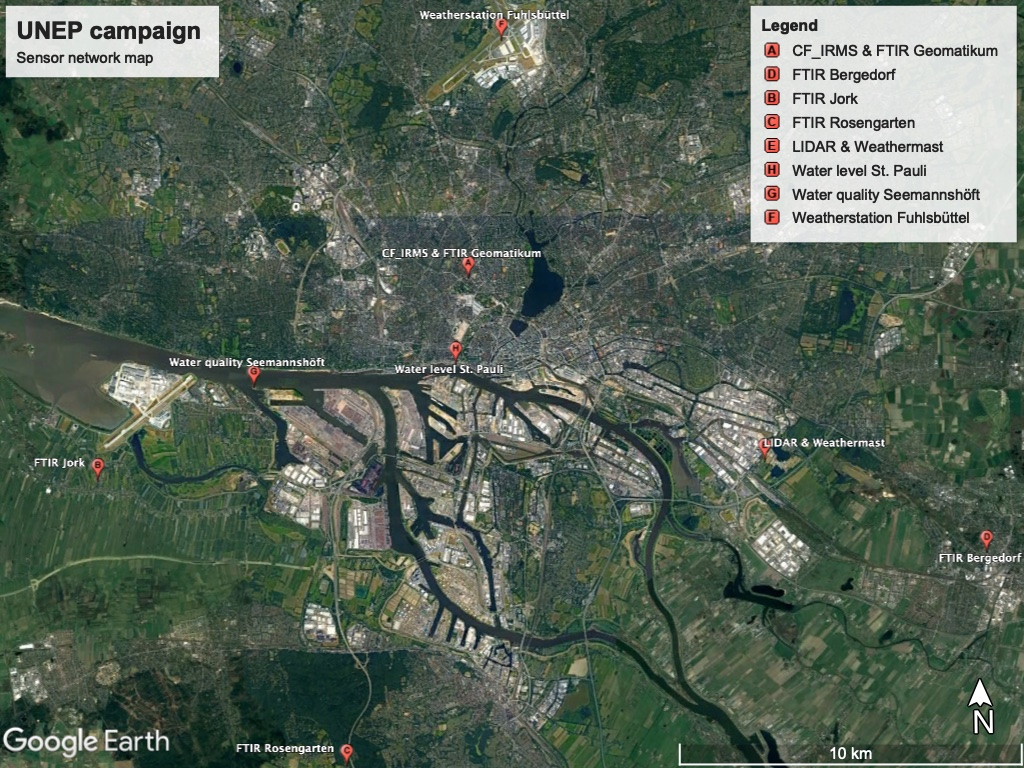
\includegraphics[width=1\textwidth]{figures/Appendix/Map/UNEP_map.jpg}
 \caption[UNEP Map of sensor network]{Satellite image of Hamburg with the location of the sensors deployed in the UNEP measurement campaign marked on the map. A: Geomatikum of University Hamburg with CF-IRMS, FTIR and Wind measurements, B: West FTIR station in Jork, C: South FTIR station in Rosengarten, D: East FTIR station in Bergedorf, E: Weather mast and Wind LIDAR both measuring wind in Billbrook, F: DWD Weather station Fuhlsbüttel, G: Water quality measurements at Seemennshöft, H: Water level measurements at St. Pauli. \cite{GoogleLLC.2023}}
 \label{UNEPmap}
\end{figure}
The enclosures operate by measuring the absorption infrared solar spectrum with a high temporal resolution of 90 seconds, which is later used in the retrieval process, averaged over a 10 min period to accurately calculate the CO$_2$, CH$_4$, and O$_2$ the column integrated dry air mole fractions. \\
The enclosures are equipped with a Michelson interferometer (Bruker, EM27/Sun). This spectrometer has an attached solar tracker that enables the tracking of the Sun by redirecting the light rays with a set of electronically controlled gold-plated mirrors. The spectrometer is housed in a weatherproof aluminium box to protect it and its auxiliary equipment, such as a computer, heating unit, control electronics, etc., from the elements. To enable an undisturbed light ray, the solar tracker sticks out the top of the box with an automatic cover that opens at favourable weather conditions and aligns itself with the solar tracker. To protect the tracker from precipitation, a rain sensor and a cloud detection sensor are placed on top of the enclosure. They automatically initiate a closure of the cover when precipitation is detected, or the cloud coverage is too great. The weatherproof enclosure and automated operation allow for autonomous data acquisition of a geographically extensive network with minimal staffing. Data collection during fluctuating weather conditions can be achieved as the measurement can be initiated and terminated quickly without lengthy setup times.
\begin{figure}[htbp]
 \centering
 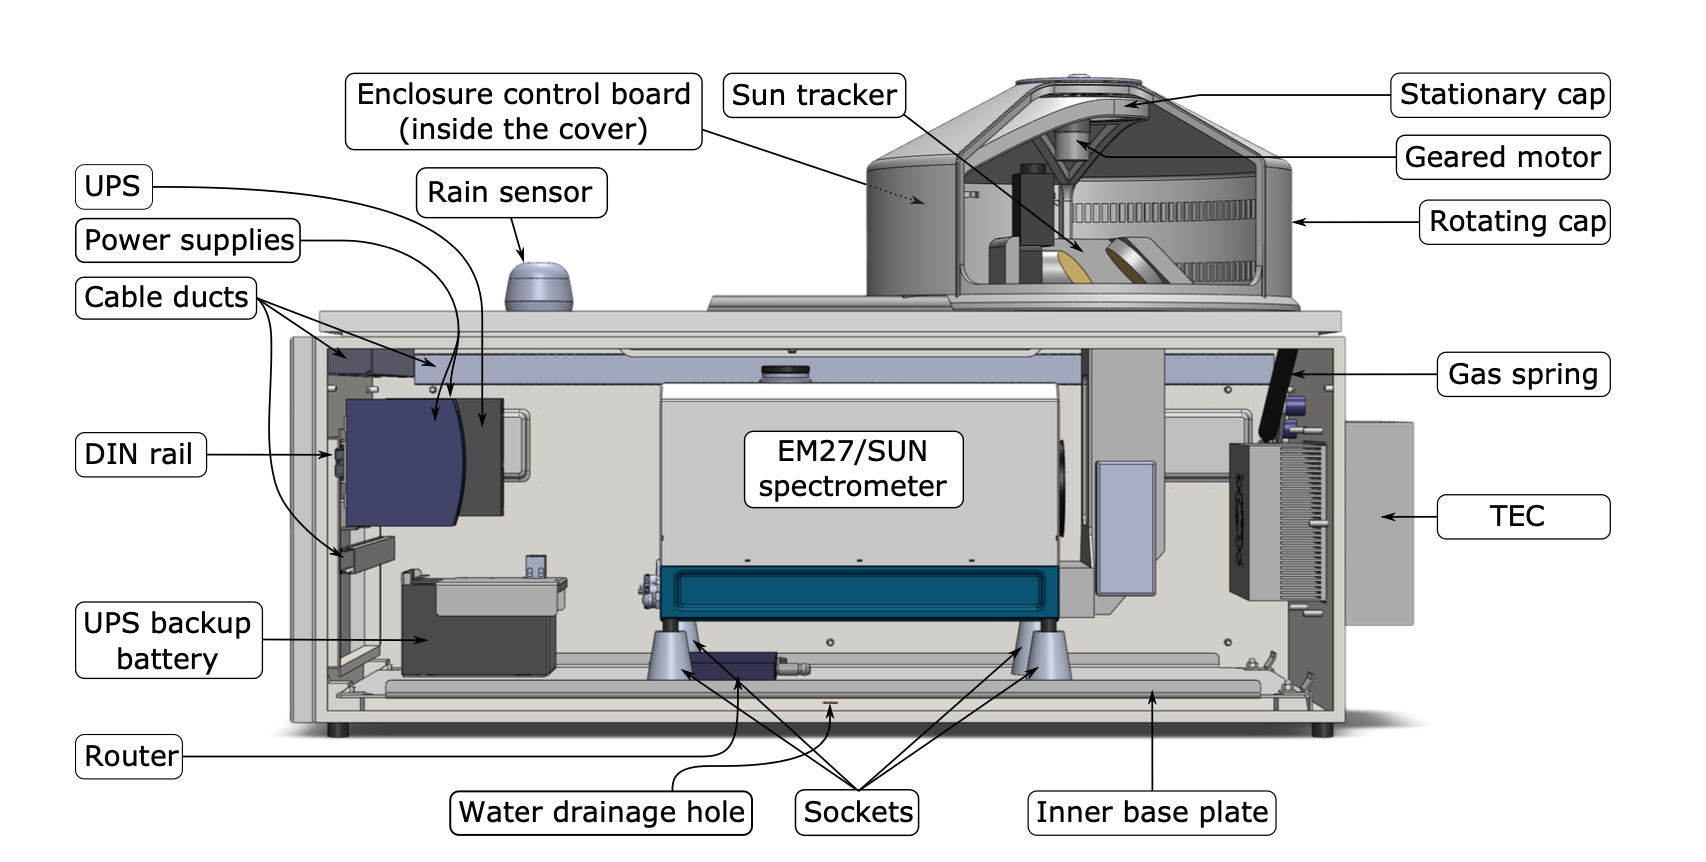
\includegraphics[width=1\textwidth]{figures/Methode/FTIR_Enclousure_schematics.png}
 \caption[FTIR spectrometer enclosure schematics]{Schematics of the FTIR spectrometer enclosure (MUCCnet). \cite{Heinle.2018}}
 \label{FTIRSchematics}
\end{figure}
The significant advantage of the FTIR approach to other in situ measurements lies in the total column measurement, which measures the total air column of the atmosphere between the light emitter, i.e. the sun and the spectrometer. The spectral absorption by the methane can then accurately be measured for the entire atmosphere. Other approaches that measure concentration at the street level have the disadvantage that they can miss methane emission emitted above the instruments like high chimneys. The degree of mixing of the GHG with the background air highly depends on various airflow characteristics, topography, emission type, and location. A total column measurement can’t negate all of them, but it gives a more reliable picture than simple in situ measurements. 

\subsection{Bayesian inversion modeling}
By using the FTIR sensor network,  differential total column measurements were performed, in which at least one sensor is always located upwind and one downwind of an emitter. The quantity of GHG released by an emitter can be estimated by comparing the concentration delta of the two columns.\\
A computational fluid dynamics (CFD) model is used to identify the emission location. This is aided by using a Bayesian inversion framework.\\
An inverse Framework is a method where the effects of an event or condition are used to calculate the cause that leads to the observed effects. Here the methane concentration was measured in the atmosphere, and it is attempted to calculate its emitters. In a forward method, the measured concentration in the air would be calculated from the known emitters.\\
To statistically improve the calculation of the cause, further prior information can be used. The TNO inventory, which has the highest spatial resolution of “known” emitters in Hamburg, is used in this case. This inventory is compiled by estimating emissions due to fossil fuel usage, density, type of emission, etc.
When applying the Bayesian approach in the Inversion, the TNO GHGco inventory was used as the prior estimation of the emissions.\\
The TNO GHGco Inventory is a European database with spatially resolved emission data for CO$_2$, CH$_4$, CO, NOx and NMVOCs. The spatial resolution is (1/60)◦ for longitude and (1/120)◦ for latitude” \cite{Super.2020} \cite{Super.2019}. This inventory is Hamburg's current highest resolution inventory, giving the best available prior emission estimation. Its limitation is that the Bottom-up approach may not encounter all emission sources or does not yet account for relocated and sporadic emitters. To further improve the inventory, an additional layer that contained estimated emissions from the Elbe was added. For this estimation of methane emissions from the separate sections of the Elbe by \cite{Matousu.2017} were added for each grid cell individually. Each grid cell was multiplied by the proportion of water coverage in this cell to account for the incomplete coverage of the Elbe by coarse raster \cite{Forstmaier.2023}.\\
In Bayes’s theorem, the posterior model is proportional to the prior model, which is the probability of the methane being emitted using previously acquired knowledge times the “likelihood of the Data”. The likelihood of the Data links the target model (the posterior of the measured variable) to the measured data. The likelihood is the probability of measuring a concentration given the emission from the Prior model.
\begin{equation}
Posterior probability = \frac{Prior probability * Likelihood of the data}{Normalization constant}
\end{equation}
\begin{equation}
P(A|B) = \frac{P(B|A)P(A)}{P(B)}
\end{equation}
A Bayesian inversion can estimate the methane emission of a source by using prior knowledge of the source by updating this knowledge with measurements of the methane concentration in the air.\\
To identify the locations, the Inversion also uses the ERA5 weather model. This model is additionally corrected for the boundary layer height and wind direction using a wind LIDAR. This corrected model is then used to generate backward trajectory footprints with a Stochastic Time-Inverted Lagrangian Transport (STILT) model. The Inversion is then able to use the STILT footprints for its identification of the emission location. For the UNEP campaign, the existing framework developed by \cite{Jones.2021} was adopted for Hamburg and used in the analysis.

\section{Peak identification algorithm}
The Isotope ratio mass spectrometer measurements show a series of methane concentration peaks throughout the campaign time, with different magnitudes and durations. Hence the identification and characterisation of the peaks were of great importance. To achieve this goal, a peak finder algorithm was implemented that identifies the methane peaks over the entire time series. Outputting the maximal concentration and its time, together with the peaks start and end time and concentrations. The peak finding algorithm was tuneable in its identification criteria, allowing for separate investigations. With the peak identification, an automated tool was provided to be used later in the pipeline for isotope signature identification and correlation with other variables.\\
In the analysis, two different identification criteria were consequently used. The first was the identification of all methane peaks that are distinct from the background concentration. The identification criteria defined by \cite{Menoud.2021} were used as a reference. The following criteria were applied:
\begin{itemize}
  \item A minimum enhancement above the background of 100 ppb.
  \item A minimum peak height of the lowest 10th percentile of the concentration-time series.
  \item The peak width contains at least 3 data points (approximately 60min).
  \item The peak width is restricted to maximum ± 6 hours around the centre of the peak.
\end{itemize}
Figure \cref{TimelinePeaksPaper} shows an example of the peaks with the identified peak highlighted.\\
The second peak identification criteria are designed to identify only the short and very prominent peaks. Those peaks are visually different from most others, and a different production mechanism was suspected. The peculiarity of those peaks was separately investigated to identify the mechanisms that govern those peaks. The criteria applied are as follows:
\begin{itemize}
  \item High concentration of min 2100 ppb.
  \item Min 3 data points.
  \item Shorter max peak spared of 3 h.
\end{itemize}
An example of the identified peaks can be seen in \cref{TimelineMediumPeaks}. 

\section{Methane and environmental data correlation analysis}
\subsection{Methane emissions with water level}
At first inspection, the presence of the methane peaks in the concentration timeline occurs at random. Overlaying the methane concentration with the water level measurements at St. Pauli in Hamburg, provided by Bundesanstalt für Gewässerkunde (BfG), indicates a correlation.
A pattern can be spotted in Figure Plot \cref{TimelineCH4Waterlevel}, which is a section of the complete timeline. The dominant methane peaks occur around 1-3 h after the lowest water level. \\
While smaller peaks are visually more challenging to identify and correlate to the Water level, the peak identification algorithm helps to highlight the smaller peaks. It further indicates a correlation with the water level of the river Elbe. \\
Pearson's correlation coefficient was used to prove a statistically meaningful correlation between the water level and the methane concentration. Unfortunately, the occurrence of elevated methane concentrations doesn’t seem to be a single variable correlation. So, a simple correlation of the total water level and concentration yields no correlation. \\
The wind direction must be considered to establish a correlation between water level and methane. This was done by separating the timeline in wind directions and speeds to be analysed separately by binning all methane and water level measurements in 10° Wind directions and 1 m/s wind speed bins. Followed by calculating the Pearson's correlation coefficient between the water level and methane concentration in the air for each bin.\\
A visual representation of the obtained results can be seen in Plot \cref{WaterLevelPCCGeomatikum}. Each tile in this plot represents a wind data bin, with the colour representing Pearson's correlation coefficient.\\
It can be seen that in three regions with particular directions and speeds, a strong correlation between methane and the water level is observed.\\
To validate if the correlations are statistically meaningful, a p-value test has also been conducted with a value of $<$0.05. A plot visualizing the results can be seen in \cref{WaterLevelCorrPValueGeomatikum}.\\
Fortunately, the Regions of interest pass the test, while the regions that don’t show a correlation to the water level fail the test as expected.

\subsection{Methane concentration and water quality correlation}
It is well known that wetlands and waterbodies can release significant amounts of methane into the atmosphere. \cite{Matousu.2019} show that a high methane concentration in the water of the Elbe is present in the upper estuary of the city of Hamburg. The TNO GHGco inventory does not include emissions from the river Elbe, but \cite{Forstmaier.2023} shows that a correction including estimations of the river's emissions yields more reliable modelling results.\\
Water quality parameters are a good indicator of methane production, reduction and emission rates in the water \cite{Wu.2007}.  A direct methane emission prediction cannot be made just from such water quality parameters due to the complexity of the production mechanism and its strong dependence on local conditions and microbial composition present in the water body. Nether the less, a correlation between water quality parameters and methane production was observed. This can help to provide further indication of alleviated methane concentration in the air due to mechanisms in the water of the river Elbe. \\
To investigate if the methane peaks and the methane concentration in the air are connected to the river Elbe, the water quality parameters of the Elbe have been correlated with the methane concentration time series.\\
The water quality data measured at Elbe Seemannshöft provided by Hamburg Service were used \cite{IHUW.20230501}. This data included the parameters: Water temperature, Oxygen concentration and saturation, pH-value, conductivity $\kappa$25, turbidity, UV-absorption SAK and algae concentration of different types. The data had a high temporal resolution of 10 min. \\
A Pearson's correlation coefficient analysis was made using the same correlation approach described before for the same wind direction and speed bins. An example can be seen in \cref{CorrelationWaterQuality}.

\subsection{Methane concentration and meteorological observations correlation.}
The release of methane into the atmosphere by natural and anthropogenic mechanisms is highly dependent on environmental conditions. These include, for example, meteorological parameters such as temperature, precipitation, and solar intensity.\\
For natural methane emissions, methane production and release into the atmosphere depend highly on temperature. Different microbes have a preferred temperature at which their methane production or reduction mechanisms peak. Higher temperatures are generally favourable for methane production \cite{Singh.2000}. Another significant parameter is the precipitation amount and consequent water abundance on the surface. Some microbes live in water or moist environments. An abundance of surface water aids the population growth of such microbes. Additionally, water can help to flush organic material into the waterbody providing a plethora of nutrition for the microbes, allowing for a large population and methane production. \\
Anthropogenic methane production is differently affected by meteorological parameters as the behaviour of humans mainly governs it. A well-observed example is the increase in fossil fuel consumption at colder temperatures \cite{Javadinejad.2019}. This is primarily observed in an annual cycle. Methane from anthropogenic sources is often released into the atmosphere through leaks in the infrastructure or incomplete combustion. Other parameters and mechanisms also exist and are primarily dependent on the environment.\\
It was attempted to investigate a possible correlation between the methane concentration in the air and some meteorological parameters.  The Deutsche Wetteredienst (DWD) data was used for this. The measurement station Hamburg-Fuhlsbüttel was used due to its proximity to the Geomatikum (2.3 km). This Station provides highly standardised and quality-controlled measurement data, which were 10 min and 1 h averaged by the DWD \cite{Kaspar.2013}.\\
The measurement parameters investigated were: air temperature at 2 m, dew point, humidity, precipitation, air pressure, and solar radiation intensity.\\
The correlation investigation was performed in a similar manner as with the water quality and water level. A Pearson's correlation coefficient analysis and a P-value test for separate wind direction and speed bins, the resulting correlations were plotted in a tile plot for better visualisation.

\section{Methane transport by wind}
\subsection{Methane emissions and wind measurements}
As previously mentioned, the wind plays a significant role in the measured methane concentration at the Geomatikum. Hence a detailed analysis of the observed wind is essential. The wind data from the Deutsche Wetterdienst (DWD) and Universität Hamburg was used in this thesis. \\
The Deutscher Wetterdienst (DWD) provides weather and climate data throw their Open Data Climate program \cite{DeutschenWetterdienst.20230501}, with an extensive array of measured parameters at different measurement time intervals for a large selection of weather stations. In Hamburg alone, there are two Stations and about five near the city. In this thesis, the data from the Fuhlsbüttel, Hamburg Station, has been used due to the proximity to the Geomatikum, where the CR-IRMS and one of the FTIR spectrometer stations were located. \\
A significant advantage of using the data provided by the DWD is the standardization and quality control done by the DWD, providing considerable confidence in the measurements. Additionally, the wide arrange of measured parameters provided, including, for example, precipitation, soil and air temperature, solar radiation intensity, etc., enables comparison and correlation with many aspects of methane emission.\\
While this data adheres to strict standards, the wind measurements are performed only 2 m above ground. Measurements of this altitude are heavily influenced by surrounding topography. While time averaging helps in normalising the measurement, it does impact the temporal resolution of the measurements.\\
The Universität Hamburg provided three different sets of wind measurements at two locations \cite{Lange.20220501}. The first location was at the Geomatikum itself, only a few metres from the CF-IRMS measurement inlet at the height of 83 m. At this height, the surface-level effects are mostly negated. But the Geomatikum building itself can potentially generate turbulences that influence the measurements. The Geomatikum was the highest building in the proximity by quite a margin, but disturbances from the surrounding can’t be completely out-ruled. The second location is at the weather mast in Hamburg Billbrook, about 17.3 km East of the Geomatikum. Measurements there were made at the height of 50m and 110m. The measurement instruments are placed far from the support structure so that disturbances by the mast are minimised. Additionally, no high-rise buildings are located near the mast, aiding a mostly undisturbed measurement.\\
All four measurement data sets were time averaged over 10 min, and all were analysed and used in further modelling. The measurements at the Geomatikum proved to be the most reliable data set, and the analysis in this thesis mainly focuses on it. The proximity to the isotope measurement inlet was the main contributor to the reliability, as small local wind patterns were picked up by both measurements simultaneously. 

\subsection{Methane emission distance modelling}
In the methane concentration time series at the Geomatikum, the prominent peaks are very sharp, with a relatively short duration of 0.5 to 3 h and a very high methane concentration of up to 4000 ppb for a background concentration of 2000 ppb. This indicates an emitter located nearby with a relatively short emission time and a high amount of methane released. \\
To estimate the Distance between the emitter and the measurement location,
the strong correlation between the methane concentration in the air and the tidal cycle of the Elbe is used.
To achieve this, virtual tracks of wind particles are modelled using the wind data measured at the Geomatikum. \\
%check and rewrite the Elipsodial disatance formular plus add reference
The tracks are modelled for the time between the maximal methane concentration of a peak and the lowest water level during the low water cycle of the Elbe before the methane peak. Tracks are backwards-modelled in time, originating at the Geomatikum. The particle follows the measured wind, with a time resolution of 10 min as dictated by the measurement. At each 10 min interval, the partial location is calculated using its previous location, the wind data and Bowring's Ellipsoidal-surface formulae.  This is repeated until the time when the lowest water level is reached. The total 
Geodesics distance between the Geomatikum and the final location, i.e. the estimated emission location, is then calculated. The resulting distance for all peaks is plotted versus its peak's maximal methane concentration in a scatterplot. This can be seen in \cref{DistancePlot}.

\subsection{Gaussian plume transport modelling for methane peaks}
A transport model was constructed to locate the emission regions causing the prominent methane peaks. For this purpose, the temporally high-resolution wind data provided by the University of Hamburg and the Deutsche Wetterdienst (DWD) have been used. The transport model uses the wind data to create Gaussian plumes with the measurement site as a particle emitter.\\
The emitted particles travel backwards in time; this allows the calculation of reversed particle tracks. To create Gaussian plumes at a specific emission time, many particles are emitted simultaneously at this time. The particle tracks are calculated using the wind direction and speed for each wind measurement interval. So that the particle can follow changes in wind direction and speed over time. The direction and speed of each particle are randomised with a predetermined Standard deviation at each interval for each particle. The degree of randomisation was taken from literature values for similar topography and wind speeds as in Hamburg (SD wind speed 0.5 m/s, SD wind direction = 20° \cite{Farrugia.2017}). The standard deviation was calculated for each wind measurement dataset using the rolling Yamartino method for the wind direction and a normal standard deviation for the wind speed showed similar values for all datasets. As a large number of particles are emitted, the randomisation on each individual particle yields a Gaussian distribution for the total particle distribution.\\
The transport model was used in tandem with the peak finding algorithm to investigate the peak methane emission locations. After the methane peaks are identified, the time of lowest water level is within 12 h before the methane peak is identified. 
Around half an hour before the lowest water level, the majority of the shallow water regions of the Elbe are completely water-free, exposing the soil and sediments to the air. Those regions can be seen in \cref{TopographyElbeHamburg}, showing a topographic map of the Elbe  in Hamburg. The Regions that dry out during a low tide start from 0m (yellow) to 2.7 m (red). It has to be noted that this survey does not include all connected channels and Fleeds surrounding the Elbe. Most are located in and around the city centre, and all of them are exposed during low tide. To account for all the sections of the river that dry out before the lowest water level is attained, Half an hour before the lowest water level is calculated. It is estimated that at this time, the majority of the shallow regions are dry, but due to the change in the tidal range over a lunar cycle, this can vary substantially.
\begin{figure}[htbp]
 \centering
 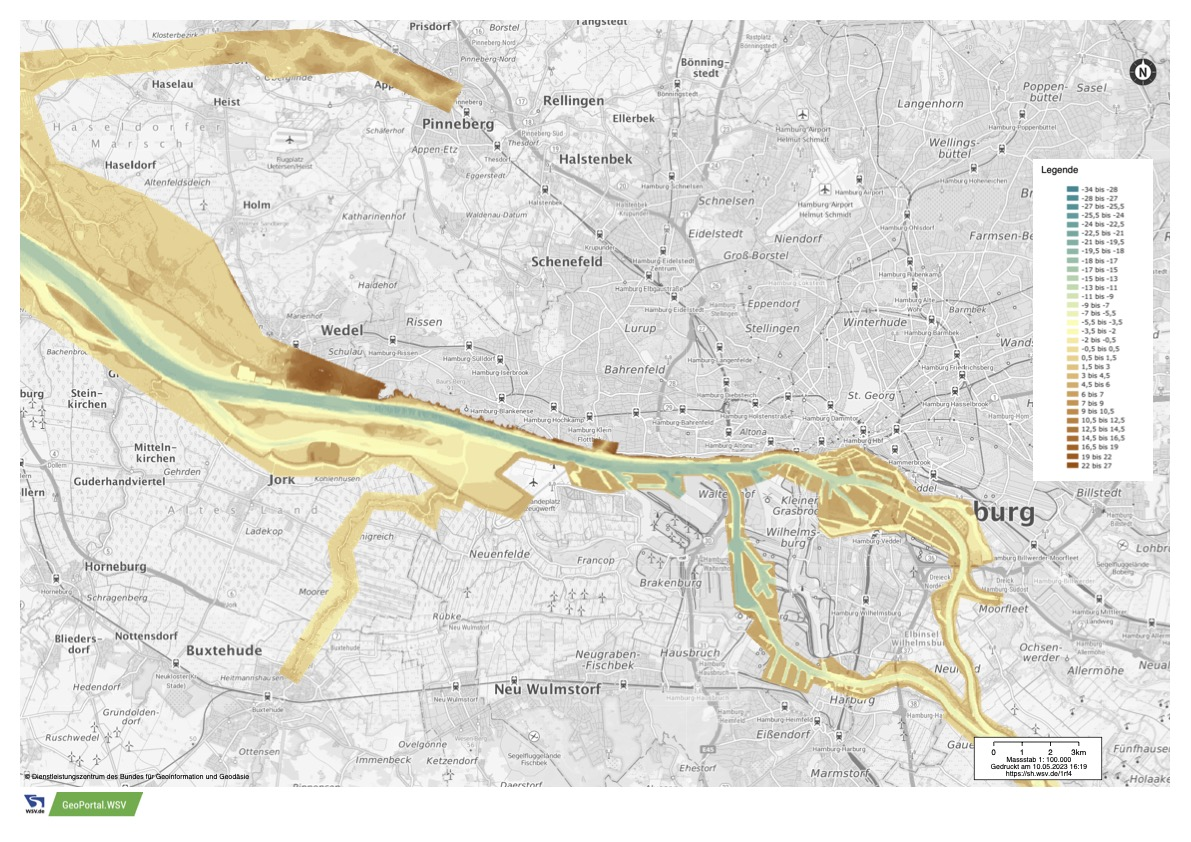
\includegraphics[width=1\textwidth]{figures/Appendix/Map/TopographieElbeHamburg.jpg}
 \caption[Topographic map of Elbe in Hamburg]{Topographic map of the river Elbe in the Hamburg region, Scale is in dm, 0 dm is at mean sea level. \cite{ZDMGDWS.2016}}
 \label{TopographyElbeHamburg}
\end{figure}
The particle tracks are only calculated for the time between this half hour before the lowest water level and the maximum methane peak. \\
After all particle tracks for all selected emission times are completed, the particle distribution density is calculated. This is done by splitting the map into a 1000x1000 segment raster and calculating the density of particles in each segment. The raster is then normalised for the total domain. The transport model outputs a map with the rasterised particle density overlay as an interactive map \cref{TransportmodelStrictPeaks}.\\
Using this approach, it can be observed that many particle tracks follow the path of the  Elbe quite closely. 

